%----------------------------------------
\begin{frame}
  \frametitle{Part 6}

\iconllm[3.2]

\vspace{0.45cm}

{\Large\bf LLMs: writing the model was always the expensive part}

\end{frame}

%----------------------------------------
\begin{frame}
  \frametitle{Who wrote the queue model?} \small

Twelve man-weeks for the Remote Agent model. That cost --- not the checking --- is
why formal methods stayed a specialist activity.

\pause
\vspace{0.3cm}

The lock-free queue in Part 4 went differently. An LLM reading the pull request
{\bf flagged} the counter as suspicious; asked to demonstrate it, it {\bf wrote the
\promelaname{} model}. \spin{} then did what \spin{} does.

\vspace{0.4cm}

{\centering
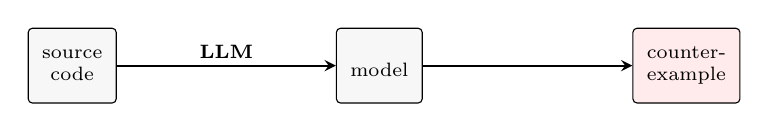
\begin{tikzpicture}[
  font=\scriptsize, >=stealth,
  box/.style={draw, rounded corners=1.5pt, align=center, inner sep=5pt,
              minimum height=0.95cm, fill=black!3},
  lab/.style={font=\scriptsize\bfseries, inner sep=2pt}
]
  \node[box] (code)  at (0,0)    {source\\code};
  \node[box] (model) at (3.9,0)  {\promelaname{}\\model};
  \node[box, fill=red!8] (cex) at (7.8,0) {counter-\\example};

  \draw[->, thick] (code)  -- node[lab, above] {LLM}    (model);
  \draw[->, thick] (model) -- node[lab, above] {\spin{}} (cex);
\end{tikzpicture}\par}

\pause
\vspace{0.3cm}

\begin{block}{}\small
\centering
The LLM proposes. The model checker disposes.
\end{block}

An LLM asserting that code is correct is worth little. An LLM producing an
artifact that a {\bf sound tool} then checks is worth a great deal --- and if the
model is wrong, the counterexample is concrete enough to see that it is wrong.

\end{frame}
